\begin{frame}{Giới thiệu Microservice}
% \begin{frame}{So sánh Kiến trúc Monolith và Microservices}
\begin{figure}[H]
\centering
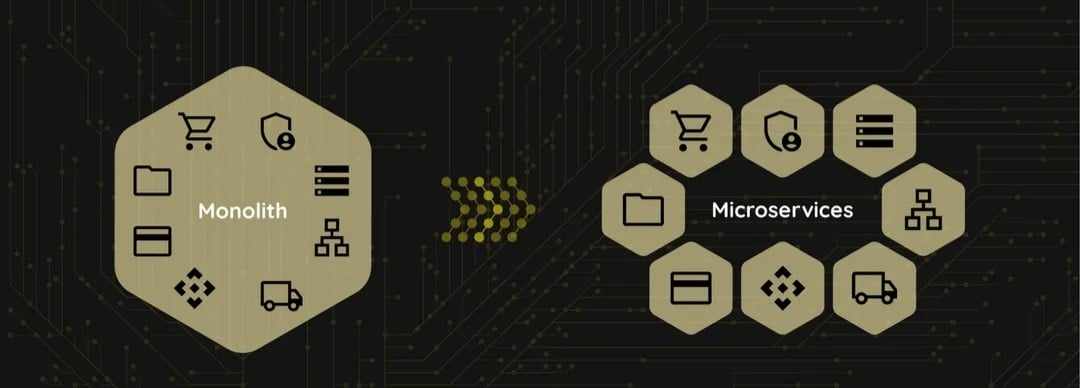
\includegraphics[height=0.55\textheight,width=0.9\textwidth,keepaspectratio]{pictures/mono.png}
\caption{Giới thiệu Microservice}
\end{figure}

\note{
Hình ảnh minh họa sự khác biệt giữa kiến trúc Đơn khối (Monolithic) và kiến trúc Vi dịch vụ (Microservices).
Kiến trúc đơn khối gộp chung tất cả các chức năng vào một ứng dụng duy nhất, gây khó khăn khi mở rộng và bảo trì. Trong khi đó, kiến trúc vi dịch vụ chia nhỏ hệ thống thành các dịch vụ độc lập, giao tiếp với nhau qua mạng, giúp tăng khả năng chịu lỗi và dễ dàng phát triển độc lập.
}
\end{frame}
